\documentclass[11pt,a4paper,]{article}
\usepackage{lmodern}

\usepackage{amssymb,amsmath}
\usepackage{ifxetex,ifluatex}
\usepackage{fixltx2e} % provides \textsubscript
\ifnum 0\ifxetex 1\fi\ifluatex 1\fi=0 % if pdftex
  \usepackage[T1]{fontenc}
  \usepackage[utf8]{inputenc}
\else % if luatex or xelatex
  \usepackage{unicode-math}
  \defaultfontfeatures{Ligatures=TeX,Scale=MatchLowercase}
\fi
% use upquote if available, for straight quotes in verbatim environments
\IfFileExists{upquote.sty}{\usepackage{upquote}}{}
% use microtype if available
\IfFileExists{microtype.sty}{%
\usepackage[]{microtype}
\UseMicrotypeSet[protrusion]{basicmath} % disable protrusion for tt fonts
}{}
\PassOptionsToPackage{hyphens}{url} % url is loaded by hyperref
\usepackage[unicode=true]{hyperref}
\hypersetup{
            pdftitle={Expert advice from experts},
            pdfborder={0 0 0},
            breaklinks=true}
\urlstyle{same}  % don't use monospace font for urls
\usepackage{geometry}
\geometry{a4paper, centering, text={16cm,24cm}}
\usepackage[style=authoryear-comp,]{biblatex}
\addbibresource{references.bib}
\usepackage{longtable,booktabs}
% Fix footnotes in tables (requires footnote package)
\IfFileExists{footnote.sty}{\usepackage{footnote}\makesavenoteenv{long table}}{}
\IfFileExists{parskip.sty}{%
\usepackage{parskip}
}{% else
\setlength{\parindent}{0pt}
\setlength{\parskip}{6pt plus 2pt minus 1pt}
}
\setlength{\emergencystretch}{3em}  % prevent overfull lines
\providecommand{\tightlist}{%
  \setlength{\itemsep}{0pt}\setlength{\parskip}{0pt}}
\setcounter{secnumdepth}{5}

% set default figure placement to htbp
\makeatletter
\def\fps@figure{htbp}
\makeatother


\title{Expert advice from experts}

%% MONASH STUFF

%% CAPTIONS
\RequirePackage{caption}
\DeclareCaptionStyle{italic}[justification=centering]
 {labelfont={bf},textfont={it},labelsep=colon}
\captionsetup[figure]{style=italic,format=hang,singlelinecheck=true}
\captionsetup[table]{style=italic,format=hang,singlelinecheck=true}


%% FONT
\RequirePackage{bera}
\RequirePackage[charter,expert,sfscaled]{mathdesign}
\RequirePackage{fontawesome}

%% HEADERS AND FOOTERS
\RequirePackage{fancyhdr}
\pagestyle{fancy}
\rfoot{\Large\sffamily\raisebox{-0.1cm}{\textbf{\thepage}}}
\makeatletter
\lhead{\textsf{\expandafter{\@title}}}
\makeatother
\rhead{}
\cfoot{}
\setlength{\headheight}{15pt}
\renewcommand{\headrulewidth}{0.4pt}
\renewcommand{\footrulewidth}{0.4pt}
\fancypagestyle{plain}{%
\fancyhf{} % clear all header and footer fields
\fancyfoot[C]{\sffamily\thepage} % except the center
\renewcommand{\headrulewidth}{0pt}
\renewcommand{\footrulewidth}{0pt}}

%% MATHS
\RequirePackage{bm,amsmath}
\allowdisplaybreaks

%% GRAPHICS
\RequirePackage{graphicx}
\setcounter{topnumber}{2}
\setcounter{bottomnumber}{2}
\setcounter{totalnumber}{4}
\renewcommand{\topfraction}{0.85}
\renewcommand{\bottomfraction}{0.85}
\renewcommand{\textfraction}{0.15}
\renewcommand{\floatpagefraction}{0.8}


%\RequirePackage[section]{placeins}

%% SECTION TITLES


%% SECTION TITLES
\RequirePackage[compact,sf,bf]{titlesec}
\titleformat*{\section}{\Large\sf\bfseries\color[rgb]{0.7,0,0}}
\titleformat*{\subsection}{\large\sf\bfseries\color[rgb]{0.7,0,0}}
\titleformat*{\subsubsection}{\sf\bfseries\color[rgb]{0.7,0,0}}
\titlespacing{\section}{0pt}{2ex}{.5ex}
\titlespacing{\subsection}{0pt}{1.5ex}{0ex}
\titlespacing{\subsubsection}{0pt}{.5ex}{0ex}


%% TITLE PAGE
\def\Date{\number\day}
\def\Month{\ifcase\month\or
 January\or February\or March\or April\or May\or June\or
 July\or August\or September\or October\or November\or December\fi}
\def\Year{\number\year}

%% LINE AND PAGE BREAKING
\sloppy
\clubpenalty = 10000
\widowpenalty = 10000
\brokenpenalty = 10000
\RequirePackage{microtype}

%% PARAGRAPH BREAKS
\setlength{\parskip}{1.4ex}
\setlength{\parindent}{0em}

%% HYPERLINKS
\RequirePackage{xcolor} % Needed for links
\definecolor{darkblue}{rgb}{0,0,.6}
\RequirePackage{url}

\makeatletter
\@ifpackageloaded{hyperref}{}{\RequirePackage{hyperref}}
\makeatother
\hypersetup{
     citecolor=0 0 0,
     breaklinks=true,
     bookmarksopen=true,
     bookmarksnumbered=true,
     linkcolor=darkblue,
     urlcolor=blue,
     citecolor=darkblue,
     colorlinks=true}

\usepackage[showonlyrefs]{mathtools}
\usepackage[no-weekday]{eukdate}

%% BIBLIOGRAPHY

\makeatletter
\@ifpackageloaded{biblatex}{}{\usepackage[style=authoryear-comp, backend=biber, natbib=true]{biblatex}}
\makeatother
\ExecuteBibliographyOptions{bibencoding=utf8,minnames=1,maxnames=3, maxbibnames=99,dashed=false,terseinits=true,giveninits=true,uniquename=false,uniquelist=false,doi=false, isbn=false,url=true,sortcites=false}

\DeclareFieldFormat{url}{\texttt{\url{#1}}}
\DeclareFieldFormat[article]{pages}{#1}
\DeclareFieldFormat[inproceedings]{pages}{\lowercase{pp.}#1}
\DeclareFieldFormat[incollection]{pages}{\lowercase{pp.}#1}
\DeclareFieldFormat[article]{volume}{\mkbibbold{#1}}
\DeclareFieldFormat[article]{number}{\mkbibparens{#1}}
\DeclareFieldFormat[article]{title}{\MakeCapital{#1}}
\DeclareFieldFormat[article]{url}{}
%\DeclareFieldFormat[book]{url}{}
%\DeclareFieldFormat[inbook]{url}{}
%\DeclareFieldFormat[incollection]{url}{}
%\DeclareFieldFormat[inproceedings]{url}{}
\DeclareFieldFormat[inproceedings]{title}{#1}
\DeclareFieldFormat{shorthandwidth}{#1}
%\DeclareFieldFormat{extrayear}{}
% No dot before number of articles
\usepackage{xpatch}
\xpatchbibmacro{volume+number+eid}{\setunit*{\adddot}}{}{}{}
% Remove In: for an article.
\renewbibmacro{in:}{%
  \ifentrytype{article}{}{%
  \printtext{\bibstring{in}\intitlepunct}}}

\AtEveryBibitem{\clearfield{month}}
\AtEveryCitekey{\clearfield{month}}

\makeatletter
\DeclareDelimFormat[cbx@textcite]{nameyeardelim}{\addspace}
\makeatother

\author{\sf\Large\textbf{ Marie Curie}\\ {\sf\large Nobel Prize, PhD\\[0.5cm]} \sf\Large\textbf{ Pierre Curie}\\ {\sf\large Nobel Prize, PhD\\[0.5cm]}}

\date{\sf\Date~\Month~\Year}
\makeatletter
\lfoot{\sf Curie, Curie: \@date}
\makeatother


%%%% PAGE STYLE FOR FRONT PAGE OF REPORTS

\makeatletter
\def\organization#1{\gdef\@organization{#1}}
\def\telephone#1{\gdef\@telephone{#1}}
\def\email#1{\gdef\@email{#1}}
\makeatother
  \organization{Acme Corporation}

  \def\name{Department of\newline Econometrics \&\newline Business Statistics}

  \telephone{(03) 9905 2478}

  \email{BusEco-Econometrics@monash.edu}

\def\webaddress{\url{http://buseco.monash.edu/ebs/consulting/}}
\def\abn{12 377 614 012}
\def\logo{
\includegraphics[width=6cm]{MBSportrait}}
\def\extraspace{\vspace*{1.6cm}}
\makeatletter
\def\contactdetails{\faicon{phone} & \@telephone \\
                    \faicon{envelope} & \@email}
\makeatother

%%%% FRONT PAGE OF REPORTS

\def\reporttype{Report for}

\long\def\front#1#2#3{
\newpage
\begin{singlespacing}
\thispagestyle{empty}
\vspace*{-1.4cm}
\hspace*{-1.4cm}
\hbox to 16cm{
  \hbox to 6.5cm{\vbox to 14cm{\vbox to 25cm{
    \logo
    \vfill
    \parbox{6.3cm}{\raggedright
      \sf\color[rgb]{0.00,0.00,0.70}
      {\large\textbf{\name}}\par
      \vspace{.7cm}
      \tabcolsep=0.12cm\sf\small
      \begin{tabular}{@{}ll@{}}\contactdetails
      \end{tabular}
      \vspace*{0.3cm}\par
      ABN: \abn\par
    }
  }\vss}\hss}
  \hspace*{0.2cm}
  \hbox to 1cm{\vbox to 14cm{\rule{1pt}{26.8cm}\vss}\hss\hfill}
  \hbox to 10cm{\vbox to 14cm{\vbox to 25cm{
      \vspace*{3cm}\sf\raggedright
      \parbox{11cm}{\sf\raggedright\baselineskip=1.2cm
         \fontsize{24.88}{30}\color[rgb]{0.70,0.00,0.00}\sf\textbf{#1}}
      \par
      \vfill
      \large
      \vbox{\parskip=0.8cm #2}\par
      \vspace*{2cm}\par
      \reporttype\\[0.3cm]
      \hbox{#3}%\\[2cm]\
      \vspace*{1cm}
      {\large\sf\textbf{\Date~\Month~\Year}}
   }\vss}
  }}
\end{singlespacing}
\newpage
}

\makeatletter
\def\titlepage{\front{\expandafter{\@title}}{\@author}{\@organization}}
\makeatother

\usepackage{setspace}
\setstretch{1.5}

%% Any special functions or other packages can be loaded here.


\begin{document}
\titlepage

\clearpage

\hypertarget{introduction}{%
\section{Introduction}\label{introduction}}

What positions should players stand and get a better impact on the serve return? Are there any strategies that the players used during their tennis games? As we know, the serve return is also important in tennis, however, there is lots of analysis about the tennis before and return impact analysis were not really common, mainly because the positions of the data containing the 3D position is not easy to collect and there is not too much sample for analysis. In the project, we are going to explore a model for the return impact position of the profession mal players using recently go public tracking data summaries on the ATP Tour websites of the 2D position of the ball at the time of return impact,

\hypertarget{overview-the-dataset}{%
\section{Overview the dataset}\label{overview-the-dataset}}

The data set Figure\ref{fig:datset} includes return impact for returned points in ATP singles matches for events between 2018 and 2020. There are 25 variables and 126455 observations in this data set and each observation refers to a single point within a match. From Figure\ref{fig:tidymiss}, there is no missing value in the data set, so we omit the data wrragling this step and use the data directly.

\begin{figure}
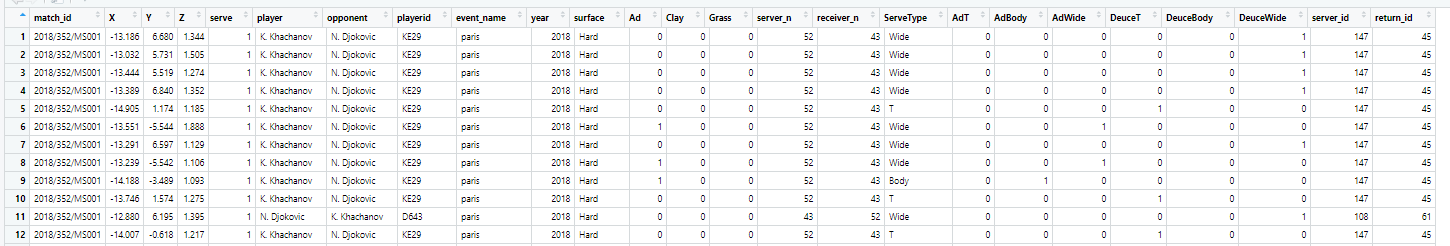
\includegraphics[width=1\linewidth]{image/dataset} \caption{Data set overview}\label{fig:datset}
\end{figure}

\begin{verbatim}
##    match_id               X                 Y                    Z         
##  Length:126455      Min.   :-23.111   Min.   :-10.587000   Min.   :-0.004  
##  Class :character   1st Qu.:-13.902   1st Qu.: -3.951000   1st Qu.: 1.191  
##  Mode  :character   Median :-12.841   Median :  0.782000   Median : 1.328  
##                     Mean   :-13.012   Mean   :  0.006236   Mean   : 1.344  
##                     3rd Qu.:-11.867   3rd Qu.:  2.903000   3rd Qu.: 1.493  
##                     Max.   : -6.423   Max.   : 10.212000   Max.   : 3.902  
##      serve          player            opponent           playerid        
##  Min.   :1.000   Length:126455      Length:126455      Length:126455     
##  1st Qu.:1.000   Class :character   Class :character   Class :character  
##  Median :1.000   Mode  :character   Mode  :character   Mode  :character  
##  Mean   :1.408                                                           
##  3rd Qu.:2.000                                                           
##  Max.   :2.000                                                           
##   event_name             year        surface                Ad        
##  Length:126455      Min.   :2018   Length:126455      Min.   :0.0000  
##  Class :character   1st Qu.:2019   Class :character   1st Qu.:0.0000  
##  Mode  :character   Median :2019   Mode  :character   Median :0.0000  
##                     Mean   :2019                      Mean   :0.4229  
##                     3rd Qu.:2020                      3rd Qu.:1.0000  
##                     Max.   :2020                      Max.   :1.0000  
##       Clay            Grass            server_n       receiver_n   
##  Min.   :0.0000   Min.   :0.00000   Min.   : 1.00   Min.   :10.00  
##  1st Qu.:0.0000   1st Qu.:0.00000   1st Qu.:16.00   1st Qu.:21.00  
##  Median :0.0000   Median :0.00000   Median :29.00   Median :32.00  
##  Mean   :0.1465   Mean   :0.05388   Mean   :28.18   Mean   :32.78  
##  3rd Qu.:0.0000   3rd Qu.:0.00000   3rd Qu.:37.00   3rd Qu.:38.00  
##  Max.   :1.0000   Max.   :1.00000   Max.   :66.00   Max.   :66.00  
##   ServeType              AdT             AdBody          AdWide      
##  Length:126455      Min.   :0.0000   Min.   :0.000   Min.   :0.0000  
##  Class :character   1st Qu.:0.0000   1st Qu.:0.000   1st Qu.:0.0000  
##  Mode  :character   Median :0.0000   Median :0.000   Median :0.0000  
##                     Mean   :0.1102   Mean   :0.138   Mean   :0.1747  
##                     3rd Qu.:0.0000   3rd Qu.:0.000   3rd Qu.:0.0000  
##                     Max.   :1.0000   Max.   :1.000   Max.   :1.0000  
##      DeuceT         DeuceBody         DeuceWide        server_id     
##  Min.   :0.0000   Min.   :0.00000   Min.   :0.0000   Min.   :  1.00  
##  1st Qu.:0.0000   1st Qu.:0.00000   1st Qu.:0.0000   1st Qu.: 50.00  
##  Median :0.0000   Median :0.00000   Median :0.0000   Median : 98.00  
##  Mean   :0.3154   Mean   :0.09277   Mean   :0.1689   Mean   : 99.94  
##  3rd Qu.:1.0000   3rd Qu.:0.00000   3rd Qu.:0.0000   3rd Qu.:151.00  
##  Max.   :1.0000   Max.   :1.00000   Max.   :1.0000   Max.   :205.00  
##    return_id    
##  Min.   : 1.00  
##  1st Qu.:21.00  
##  Median :39.00  
##  Mean   :41.05  
##  3rd Qu.:63.00  
##  Max.   :84.00
\end{verbatim}

\begin{figure}
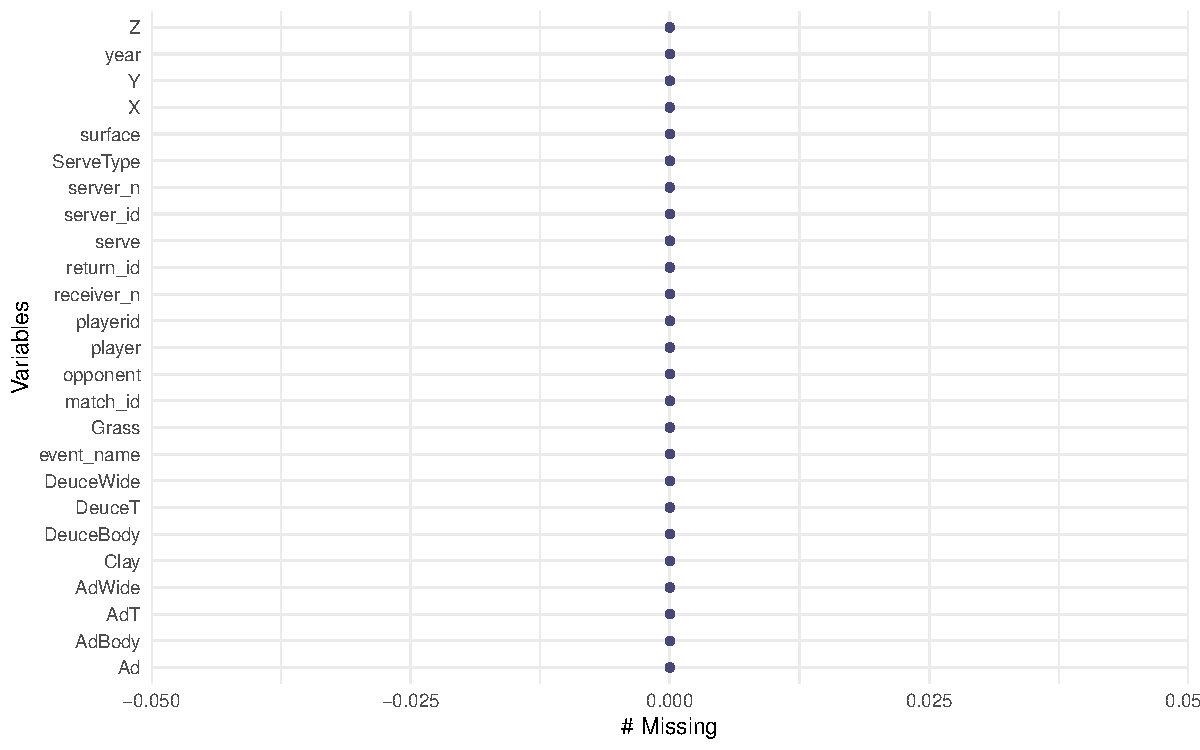
\includegraphics[width=1\linewidth]{Report_files/figure-latex/tidymiss-1} \caption{Check missing value}\label{fig:tidymiss}
\end{figure}

\hypertarget{project-goals}{%
\section{Project Goals}\label{project-goals}}

This project will develop a generative model for the return impact position of professional male players. Furthermore, the project will identify key contextual variables that may influence return impact, including but not limited to:
* Serve number
* Serve direction
* Surface
* Receiver
* Server
Moreover, there is a shiny dashboard designed for the project visualisation.

\hypertarget{how-variables-influence-players-return-impact}{%
\section{How variables influence player's return impact}\label{how-variables-influence-players-return-impact}}

\hypertarget{return-impact-model}{%
\section{Return Impact model}\label{return-impact-model}}

\hypertarget{implementation}{%
\section{Implementation}\label{implementation}}

\hypertarget{user-guide}{%
\section{User Guide}\label{user-guide}}

\hypertarget{conclusion}{%
\section{Conclusion}\label{conclusion}}

\printbibliography[title=Bibliography]

\end{document}

